\documentclass[a4paper, twocolumn]{article}

\usepackage{amsmath}
\usepackage{amssymb}
\usepackage{amsthm}
% \usepackage{bm}

\numberwithin{equation}{section}

\usepackage{float}
\usepackage{array}
\usepackage{parskip}
\usepackage{booktabs}

\usepackage[margin=2cm]{geometry}

\usepackage{siunitx}
% horrible units for fluiddynamics
\DeclareSIUnit{\kilopond}{kp}

\DeclareSIUnit{\at}{at}
\DeclareSIUnit{\ata}{ata}
\DeclareSIUnit{\atu}{at\"u}
\DeclareSIUnit{\atm}{atm}

\DeclareSIUnit{\torr}{Torr}


\usepackage{tikz}
\usetikzlibrary{calc}
\usetikzlibrary{patterns}

\usepackage{pgfplots}
\pgfplotsset{compat=1.15}
\usepgfplotslibrary{external} 
\tikzexternalize[prefix=fig/]

\usepackage{xcolor}
\usepackage[colorlinks = true,
            linkcolor = red!50!black,
            urlcolor  = blue,
            citecolor = black,
            anchorcolor = blue]{hyperref}

\usepackage{polyglossia}
\setmainlanguage{german}

 
\newtheoremstyle{hsr-def}%
    {1em}% above
    {1em}% below
    {}% body
    {0pt}% indent
    {}% headfont
    { }% headpunkt
    { }% headspace
    {\textbf{\thmname{#1} \thmnumber{#2}.} \textsc{\thmnote{#3}}}% headspec

\newtheoremstyle{hsr-sub}%
    {1em}% above
    {1em}% below
    {}% body
    {0pt}% indent
    {}% headfont
    { }% headpunkt
    { }% headspace
    {\textbf{\thmname{#1} \thmnumber{#2}.} \textsc{\thmnote{#3}}}}% headspec

\theoremstyle{hsr-def}
\newtheorem{definition}{Definition}[section]

\theoremstyle{hsr-sub}
\newtheorem{result}{Folgerung}[definition]
\newtheorem{example}{Beispiel}[definition]
\newtheorem{remark}{Bemerkung}[definition]


\newcommand{\dd}[1]{\ensuremath{\mathrm{d}#1}}
\newcommand{\di}[1]{\,\dd{#1}}
\newcommand{\deriv}[2]{\ensuremath{\frac{\dd{#1}}{\dd{#2}}}}
\newcommand{\pderiv}[2]{\ensuremath{\frac{\partial #1}{\partial #2}}}

\renewcommand{\vec}[1]{\ensuremath{\mathbf{#1}}}
\newcommand{\uvec}[1]{\ensuremath{\vec{\hat{#1}}}}

\newcommand{\unitof}[1]{\ensuremath{\left[\,#1\,\right]}}

\newcommand{\fromlecture}[1]{\textcolor{red!70!black}{\small\texttt{K.#1}}}



\begin{document}
\section{Fluide Einf\"uhrung}

\begin{definition}[Fluid]
Fl\"ussigkeiten und Gase werden under dem Oberbegriff \emph{Fluide} zusammengefasst.
\end{definition}

% \begin{description}
%     \item[Isotherm]
%     \item[Isobar]
%     \item[Isotrop]
% \end{description}


\begin{definition}[Druck und Schubspannung]
F\"ur einfache F\"alle der Cauchy Spannugstensor kann zu zwei Skalare \(p\) und \(\tau\) vereinfacht werden, sie werden Dr\"uck bzw. Schubspannung genannt.
\begin{align*}
    pA
    &= \vec{F}\cdot\uvec{n}
    = F_\perp
    &
    \tau A
    &= \vec{F}\cdot\uvec{T}
    = F_\parallel
    \stackrel{\text{statik}}{=} 0
    \\
    \unitof{p} &= \si{\newton\per\square\metre} = \si{\pascal} 
\end{align*}

\begin{result}[Gesetzt von Pascal]
In ruhenden Fluiden \(\tau = 0\), somit ist die Kraft immer senkrecht.
\end{result}

\begin{table}[h] \centering
\begin{tabular}{p{.3\linewidth} >{\(}l<{\)}}
    \toprule
    Name & \text{Einheit} \\
    \midrule
    Kilopond & \SI{1}{\kilopond} = g\,\si{\newton} \approx \SI{9.81}{\newton} \\
    Technische\newline Atmosph\"are & \begin{aligned}
        \SI{1}{\at} &= \SI{1}{\kilopond\per\square\centi\metre} \\
        &\approx \SI{0.98}{\bar}
    \end{aligned} \\
    Physikalische\newline Atmosph\"are & \SI{1}{\atm} = \SI{101325}{\pascal} \\
    Torr & \begin{aligned}
        \SI{1}{\torr} &= \SI{1/760}{\atm} \\
        &= \varrho_\text{Hg}\cdot g \cdot \SI{1}{\milli\metre}
    \end{aligned} \\
    Bar & \begin{aligned}
        \SI{1}{\bar} &= \SI{1e5}{\pascal}\\
        &\approx \SI{750}{\torr}
    \end{aligned} \\
    \bottomrule
\end{tabular}
\caption{Einheiten des Drucks}
\end{table}
\end{definition}

\begin{definition}[Dichte] Ist die Masse pro Volumeneinheit.
\[
    \varrho = \frac{m}{V} \qquad \unitof{\varrho} = \si{\kilo\gram\per\cubic\metre}
\]
\end{definition}

\section{Hydrostatik \fromlecture{1-2}}

\begin{definition}[Schweredruck]
\begin{equation} \label{eqn:hydrostatic-pressure}
    \dd{p} = \varrho \vec{g} \cdot \dd{\vec{y}} = - \varrho g \dd{y}
\end{equation}

\begin{result}[Hydrostatischer Druck]
F\"ur Fl\"ussigkeiten, da die Dichte konstant ist folgt:
\[
    p = \varrho g h
\]
\end{result}

\begin{result}[Schweredruck eines Gase]
Angenommen dass, die Dichte nur von Druck abh\"angt (barotrop)
\[
    \varrho(p) = \varrho_0 \frac{p}{p_0}
\]
Die L\"osung von \eqref{eqn:hydrostatic-pressure} ergibt die \emph{Barometrische H\"ohenformel} f\"ur eine isotherme Atmosp\"are.
\[
    p(h) = p_0 \exp\left(-\frac{\varrho_0}{p_0} gh\right)
\]
\end{result}
\end{definition}

\begin{definition}[Gesetz von Boyle-Mariotte]
% \label{def:boyle-mariotte}
F\"ur ein ideales Gas gilt bei konstanter Temperatur
\[
    pV = (\text{konstant})
\]

\begin{result}
Die Dichte ist proportional zum Druck
\[
    \frac{V_2}{V_1} = \frac{p_1}{p_2} = \frac{\varrho_1}{\varrho_2}
\]
\end{result}
\end{definition}


\begin{definition}[Kompressibilit\"at]
Die Druckerh\"ohung \(\Delta p\) bewirkt in einem Fluid stets eine Volumenabname.
Die relative Volumen\"anderung ist proportional zur Druck\"anderung
\[
    \Delta V / V = - \kappa \Delta p
\]

\begin{remark}
    Eine ideale Fl\"ussigkeit ist reibungsfrei und inkompressibel.
\end{remark}

\begin{remark}
    In einer idealen Fl\"ussigkeit ist die Dichte konstant.
\end{remark}
\end{definition}

\begin{definition}[Statische Auftriebskraft] Auch als Archimedische Prinzip bekannt.
\[
    F_A = G_f = \varrho_f  V_k g
    \qquad
    \uvec{F}_a = - \uvec{g}
\]
Der auftrieb eines in ein Fluid eingetauchen K\"orper ist gleich dem Gewicht des von ihm verdr\"angten Fluids.
\end{definition}

\subsection{Grenzfl\"acheneffekte}

\begin{definition}[Oberfl\"achenspannung]
Zwischen zwei Atomen oder Molek\"ulen tritt die \emph{Van der Waals}-Kraft.
An der Oberfl\"ache der Fl\"ussigkeit ist der mittlere Abstand der Molek\"ule etwas gr\"osser als im Innern. Das bewirkt eine Parallel zur Oberfl\"ache gerichtete anzihende Kraft zwischen den Molek\"ulen.
\[
    \sigma = \frac{F}{\ell}
    \qquad
    \unitof{\sigma} = \si{\newton\per\metre}
\]
\begin{remark}
Die Oberfl\"achenspannung kann auch als \emph{spezifische Oberf\"achenenergie} bezeichnet werden.
\[
    \sigma
    = \frac{\Delta W}{\Delta A} 
    = \frac{F\Delta s}{\ell \Delta s}
    = \frac{F}{\ell}
\]
Die \emph{Oberfl\"achenenergie} ist ein Ma{\ss} f\"ur die Energie, die zum Aufbrechen der chemischen Bindungen notwendig ist, wenn eine neue Oberfl\"ache einer Fl\"ussigkeit oder eines Festkörpers erzeugt wird.
\end{remark}

\begin{result}[Grenzfl\"achenspannung]
Bei einer Vergr\"osserung der Grenzfl\"ache muss Arbeit geleistet werden, da die Grenzfl\"achenenergie vergr\"ossert wird.
Es gibt dann auch die Grenzfl\"achenspannungen 
\(
    \sigma_\text{sl},
    \sigma_\text{sg},
    \sigma_\text{lg}
\) (fl\"ussig = liquid, fest = solid, gas) die zwischen Festk\"orper und Fl\"ussigkeit wirken. \(\varphi\) ist dann der \emph{Kontaktwinkel}, und die Geometrie ergibt die Beziehung
\[
    \sigma_\text{sg} = \sigma_\text{sl} + \sigma_\text{lg} \cos \varphi
\]
\end{result}

\begin{example}[Druck in Seifenblase]
\[
    p = \frac{2\sigma}{r}
\]
\end{example}
\end{definition}

\begin{definition}[Kapillarit\"at]
Allgemein an die Grenze gilt:
\[
    F_\text{Oberfl\"ache} = F_{G,\text{Fl\"ussigkeit}}
\]
\begin{result}[In einem Rohr (Zylinder)]
\[
    2\pi r\sigma = \varrho\pi r^2 hg \implies  h = \frac{2\sigma}{\varrho g r}
\]
\end{result}
\end{definition}

\section{Hydrodynamik}
\subsection{Einf\"uhrung \fromlecture{3-4}}
\begin{definition}[Kontinuit\"atsgleichung]
\begin{equation} \label{eqn:continuity}
    \pderiv{}{t}\int_V \varrho \di{V} 
    = \oint_{\partial V} \varrho \vec{v}\cdot\di{\vec{s}}
\end{equation}

\begin{result}[Ideales Fluid]
Da die Dichte konstant ist (inkompressibel), man kann \eqref{eqn:continuity} durch \(\varrho\) teilen und folgt:
\[
    \dot{V} = \int_A \vec{v}\cdot\di{\vec{s}} 
    = vA = \frac{\dot{m}}{\varrho}
    \qquad
    \unitof{\dot{V}} = \si{\cubic\metre\per\second}
\]
\end{result}

% \begin{remark}[Differentialform]
% \[
%     \nabla \cdot (\varrho \vec{v}) + \pderiv{\varrho}{t} = 0
% \]
% \end{remark}
\end{definition}

\begin{definition}[Bernoulli Gleichung]
Der Term \(\varrho v^2 / 2\) wird \emph{dynamische Druck} genannt.
\[
    p + \varrho g h + \frac{\varrho}{2} v^2 = (\text{Konstant})
\]

% TODO: Dyn. Druck + Stat. Druck = Staudruck zeigen: Buch p. 211 Abb. 9.6
\begin{figure}[h] \centering
    \resizebox{.9\linewidth}{!}{%
        \begin{tikzpicture}
    % axis
    % \draw[->] (-1.5,-1.5) to ++(0,5) node[anchor=south] {\(y\)};
    \draw[->] (-1,-1) to (8.5,-1) node[anchor=west] {\(x\)};
    
    % tube lines
    \draw[] (0,2) to (1,2) to[out=0, in=180] (6,3) to (7,3);
    \draw[] (0,0) to (1,0) to[out=0, in=180] (6,2) to (7,2);
    
    % opening ellipse for A1
    \draw[blue!10, fill=blue!10] (0,.025) rectangle ++(.75,1.95);
    \draw[fill=blue!10] (0,1) ellipse (.3 and 1);
    % ellipse
    \draw[dashed, fill=blue!10] (.75,1) ellipse (.3 and 1);
    % closing ellipse
    \draw[fill=blue!10] (7,2.5) ellipse (.2 and .5);
    %% hide half of the ellipse and make dashed
    \draw[blue!10, fill=blue!10] (6,2.025) rectangle ++(1,.95); 
    \draw[dashed] (7,2.5) ellipse (.2 and .5);
    % ellipse for A2
    \draw[dashed, fill=blue!10] (6,2.5) ellipse (.2 and .5);
    
    % vectors
    \draw[thick, ->] (-1,1) to node[near start, above, anchor=south] {\(v_1\)} ++(1,0) ;
    \draw[thick, ->] (5,2.5) to node[near start, below, anchor=north] {\(v_2\)} ++(1,0) ;
    
    % heights
    \draw[dotted] (0,1) to (2,1);
    \draw[->] (1.5,-1) to node[pos=.3, anchor=west, right] {\(h_1\)} (1.5,1);
    
    \draw[dotted] (6,2.5) to (8,2.5);
    \draw[->] (7.5,-1) to node[pos=.5, anchor=west, right] {\(h_2\)} (7.5,2.5);
    
    % areas
    \draw[thick, blue] (0,.4) to [out=180, in=30] node[at end, anchor=east] {\(A_1\)} ++(-.5,-.4);
    \draw[thick, blue] (6,2.2) to [out=210, in=80] node[at end, below, anchor=north] {\(A_1\)} ++(-.5,-.5);
    
    % other symbols
    \node at (3,1.5) {\(\varrho\)};
    \node at (-.7,2) {\(p_1\)};
    \node at (7.5,3) {\(p_2\)};
\end{tikzpicture}
%
    }
    \caption{Schematische Darstellung f\"ur die Bernoulli Gleichung}
\end{figure}

\begin{remark}
Bernoulli gilt f\"ur inkompressible Fluide, und gen\"ugt f\"ur Fl\"ussigkeite und Gase, sofern \(v \ll \) Schallgeschwidigkeit.
\end{remark}

\begin{result}
\begin{gather*}
    p_1 + \varrho g h_1 + \frac{\varrho}{2} v_1^2
    =
    p_2 + \varrho g h_2 + \frac{\varrho}{2} v_1^2
    \\
    \text{oder}\quad -\Delta p = \varrho g \Delta h + \frac{\varrho}{2} \Delta \left( v^2 \right)
\end{gather*}
\end{result}

\begin{result}
Wo die Geschwindigkeit am schnellsten ist, dort ist die Druck am tiefsten.
\end{result}

\end{definition}

\subsection{Reale Str\"omungen \fromlecture{5-6}}

\begin{definition}[Newton'sche Reibungsgesetz]
Die Proportionalit\"atskonstante \(\eta\) wird \emph{dynamische Viskosit\"at} oder \emph{Z\"ahingkeit} genannt.
\begin{gather*}
    \tau = \eta \deriv{v}{z}
    \stackrel{!}{=} \frac{F_\parallel}{A}  \\
    \unitof{\eta}  
    = \si{\kilo\gram\per\metre\second}
    = \si{\newton\second\per\metre}
    = \si{\pascal\second}
\end{gather*}

\begin{result}[Bernoulli Gleichung bei Newton'scher Reibung]
\[
    p_1 + \varrho g h_1 + \frac{\varrho}{2} v_1^2
    =
    p_2 + \varrho g h_2 + \frac{\varrho}{2} v_1^2 + p_\text{v}
\]
In der Praxis wird der Druckverlust \(p_\text{v}\) oft als Verlusth\"ohe \(h_\text{v}\) angegeben, d.h. diejenige H\"ohe, um die der Zufluss angehoben werden muss, um an Ausfluss aus der Stromr\"ohre denselben Druck wie im reibungsfreien Fall zu erzeugen.
\[
    p_\text{v} = \varrho g h_\text{v}  
\]
\end{result}
\end{definition}

\begin{definition}[Formel von Stokes]
(Stokes'sche Reibung) Reibungskraft einer Kugel im \"Ol 
\[
    F_R = 6\pi\eta Rv_0
\]
\end{definition}

\begin{definition}[Laminare Rohrstr\"omung]
Lauten die Gleichgewichtsbedingungen f\"ur die Kr\"afte innerhalb des Zylinders.
\begin{align*}
    F_\text{Res,Druck} - F_\text{Reib} & = 0 \\
    \pi r^2 (p_1 - p_2) - 2\pi rl\tau &= 0
\end{align*}

\begin{result}[Geschwindigkeitsverteilung] 
Innerhalb des Zylinders (\(r\) von \(0\) bis \(R\))
\[
    v(r) = \frac{\Delta p}{4\eta\ell}\left(R^2-r^2\right)
\]
\end{result}

\begin{result}[Gesetz von Hagen Poiseuille]
\begin{equation} \label{eqn:hagen-poiseuille}
    \dot{V} = \frac{\pi\Delta p R^4}{8\eta\ell}
\end{equation}
\end{result}

\begin{result}[Druckabfall]
Wenn man in \eqref{eqn:hagen-poiseuille} \(\dot{V} = \pi R^2 v\) einsetzt, folgt:
\[
    \Delta p = 32\eta\ell \frac{v}{d^2}
\]
\end{result}

\begin{remark}
Bei einer Zunahme des Rohrradius wird nicht nur die zur Verf\"ugung stehende Querschnittsfl\"ache gr\"osser, sondern zugleich w\"achst in der Rohrmitte auch die maximale Geschwindigkeit.
\end{remark}
\end{definition}

\begin{definition}[Prandtl'sche Grenzschicht]
\(D_\text{l}\) ist die Dicke der Schicht in unmittelbarer N\"ahe einer Oberfl\"ache mit L\"ange \(\ell\) an ein Fluid, der vorbeistr\"omt, der mitgezogen wird. Siehe Abb. \ref{fig:prandtl-boundary}.
\[
    D_\text{l} = \frac{\ell}{\sqrt{\mathcal{R}}} =  \sqrt{\frac{\eta\ell}{\varrho v}}
\]
\begin{figure}[h] \centering
\begin{tikzpicture}
    \pgfmathsetmacro{\k}{.8}
    \pgfmathsetmacro{\lpos}{.5} 
    \pgfmathsetmacro{\l}{5} 
    \pgfmathsetmacro{\vpos}{2}
    
    % block
    \draw[fill] (\lpos,0) rectangle ++(\l,-.2);
    \draw[<->]  (\lpos,-.4) -- node[midway, below] {\(\ell\)} ++(\l,0);
    
    % boundary line and area
    \fill [domain=0:\l, variable=\t, smooth, red!10]
        (\lpos,0)
        -- plot ({\lpos + \t},{\k*sqrt(\t)})
        -- (\lpos + \l,0)
        -- cycle;
    
    \draw[domain=0:\l, variable=\t, smooth, thick, red] (0,0)
        plot ({\lpos + \t},{\k*sqrt(\t)});
    
    % height
    \pgfmathsetmacro{\h}{\k*sqrt(\l)}
    \draw[<->] (\lpos,0) ++(\l,0) -- node[midway, right] {\(h\)} ++(0,\h);
        
    % velocity vectors
    \draw[dashed]    (\vpos,0) -- ++(0,2);
    \draw[->, thick] (\vpos, 1.5) -- node[at start, anchor=east, left] {\(v_0\)} ++(1,0);
    \draw[->, thick] (\vpos, 0.5) -- node[at start, anchor=east, left] {\(v_x\)} ++(.3,0);
    
    % text
    \node at (4,.5) {mitgezogen};
    \node at (4,2) {keine Wirkung};
    
    % axis
    \draw[->] (-.5,0) -- (\l + 1.5,0) node[anchor=west] {\(x\)};
    \draw[->] (0,-.5) -- (0,2.5) node[anchor=south] {\(y\)};
\end{tikzpicture}

\caption{Laminare Grenzschicht f\"ur eine Platte in einem Str\"omungsfeld mit Geschwindigkeit \(v_0\), und \(\ell \gg D_\text{l}\).}
\label{fig:prandtl-boundary}
\end{figure}
\end{definition}

\begin{definition}[Reynolds Zahl]
Ist ein dimensionslose Koeffizient aus der \emph{Navier-Stokes} Gleichung, der das Verh\"altnis zwischen kinetischer Energie des Fluides und dessen innerer Reibung (proportional zur Viskosit\"at) beschreibt.
\[
    \mathcal{R} = \frac{E_k}{E_r} = \frac{\varrho}{\eta} v^*\ell^*
    %\frac{\Delta p}{\tau}
\]
\(v^*, \ell^*\) sind eine charakteristische L\"ange bzw. Geschwindigkeit. Sie sind dimensionslose Variablen f\"ur geometrische und physikalische Gr\"ossen.

\begin{result}[Rohrstr\"omung]
Wird bei der Str\"omung durch ein Rohr mit kreisf\"ormigem Querschnitt der Durchmesser \(d\) als charakteristische Abmessung gew\"ahlt, somit ist die Reynolds-Zahl
\[
    \mathcal{R} = \frac{\varrho v d}{\eta}
\]
\end{result}

\end{definition}

\begin{definition}[Kritische Reynoldszahl \(\mathcal{R}_k\)]
\begin{align*}
    \mathcal{R} > \mathcal{R}_k
    \quad&\implies\quad\text{Turbulent} \\
    \mathcal{R} \leq \mathcal{R}_k
    \quad&\implies\quad\text{Laminar}
\end{align*}

\begin{result}[Kritische Reynoldszahl f\"ur die Rohrstr\"omung]
\[
    \mathcal{R}_k = 2320
\]
\end{result}

\end{definition}

\begin{definition}[Reale Rohrstr\"omung]
Turbulente Rohrst\"omung, je nach turbulent oder laminares \(\lambda\) 
\begin{equation} \label{eqn:real-ductstream}
    \Delta p = \lambda \frac{\varrho\ell}{2d} v^2
\end{equation}

\begin{example}[Turbulente \(\lambda\) nach Blasius]
\[
    \lambda_\text{t} = \frac{0.316}{\sqrt[4]{\mathcal{R}}}
\]
\end{example}

\begin{example}[Laminare \(\lambda\) nach Hagen-Poiseuille]
Das ist tats\"achlich \eqref{eqn:hagen-poiseuille} umformuliert.
\[
    \lambda_\text{l} = \frac{64}{\mathcal{R}}
\]
\end{example}
\end{definition}

\subsection{Wiederstandkr\"afte}
\begin{definition}[Auftriebskraft nach Kutta-Jukowski] Dieser Auftrieb ist eine Folgerung vom \emph{Magnus Effekt}.
\[
    F_A = \varrho v \ell \Gamma
\]
\end{definition}

\begin{definition}[Druckwiederstand]
\[
    F_D = c_W \frac{\varrho}{2}v^2 A_\perp
\]
\end{definition}

\begin{definition}[Zirkulation] Ist ein Mass f\"ur die Wirbelst\"arke.
Die Zirkulation ist eine makroskopische Gr\"osse und h\"ang vom Weg ab.
\[
    \Gamma = \oint \vec{v} \di{\vec{l}}
\]
\end{definition}

\begin{definition}[Induzierter Widerstand]
\[
    F_W = c_W^* \frac{\varrho}{2} v^2 A_\parallel
\]
\end{definition}

\begin{definition}[Dynamischer Auftrieb]
\[
    F_A = c_A \frac{\varrho}{2} v^2 A_\perp
\]
\end{definition}

\begin{definition}[Gleitwinkel]
\[
    \tan(\varphi) = \frac{F_W}{F_A} = \frac{c_W}{c_A} = \frac{v_V}{v_H}
\]
\end{definition}

\section{W\"armelehre Einf\"uhrung}
\begin{definition}[Absolute Temperatur]
\[
    T = \vartheta + \SI{273.15}{\kelvin} = \vartheta - \vartheta_0
\]
\end{definition}

\begin{definition}[Stoffmenge]
Hier \emph{Partikel} steht f\"ur Molek\"ule, Atome oder Ionen.
\[
    \SI{1}{\mole} = N_A \text{ Partikeln} = \SI{6.022e23}{\per\mole}
\]
Der Avogadro-Zahl \(N_A\) entspricht Anzahl von Partikeln in eine Mole, und 1 Mol ist als der Anzahl von Atome \textsuperscript{12}C in \SI{0.012}{\kilo\gram} definiert worden.
\end{definition}

\subsection{Fl\"ussgkeiten und Festk\"orpern}
\begin{definition}[Thermische Ausdehnung]
\begin{align*}
    \Delta \ell &= \alpha\ell\Delta T \\
    \Delta A &= \beta A \Delta T & \beta \approx 2\alpha \\
    \Delta V &= \gamma V \Delta T & \gamma \approx 3\alpha
\end{align*}

\begin{remark}[Anomalie des Wassers] Bei der Temperatur \SI{4}{\celsius} verschwindet sein Volumenausdehnungskoeffizient. Ebenfalls ungew\"ohnlich ist, dass die Dichte des festen Zustandes kleiner ist als die des fl\"ussigen Zustanges.
\end{remark}

\begin{result}[Termische Spannung]
\[
    \sigma = E\varepsilon = E\frac{\Delta \ell}{\ell} = E \alpha \Delta T
\]
\end{result}
\end{definition}

\subsection{Ideale Gase}
\begin{definition}[Universelle Gasgleichung f\"ur ideale Gase]
\begin{gather*}
    pV = nRT = n N_A k_B T = \text{ (konstant)} \\
    \text{oder} \quad \frac{p_1 V_1}{T_1} = \frac{p_2 V_2}{T_2}
\end{gather*}
\begin{itemize}
    \item \(R = N_A k_B = \SI{8.313}{\joule\per\mole\per\kelvin}\) ist die Universelle Gaskonstante
    \item \(k_B = \SI{1.381e-23}{\joule\per\kelvin}\) ist die Boltzmann-Konstante.
\end{itemize}
\end{definition}

\begin{definition}[Molzahl und Molmasse]
\[
    nM = m = \frac{N}{N_A} M
\]
wobei \(M\) ist die sogenannte Molmasse in \si{\kilo\gram\per\mole}.

\begin{result}[Spezifische Gaskonstante \(R_s\)]
\[
    pV = \frac{m}{M} RT = m R_s T
\]
\end{result}

\begin{result}[Dichte eines Gases]
\[
    \varrho = \frac{m}{V} = \frac{M}{V_m} = \frac{pM}{RT}
\]
\end{result}
\end{definition}


\subsection{Gemissche idealer Gase}
\begin{definition}[Partialdruck]
Der Druck \(p_i\) ist der Druck, den die Gaskomponente \(i\) h\"atte, wenn ihr bei der Temperatur \(T\) das ganze Volumen \(V\) zur Verf\"ugung h\"atte.
\end{definition}

\begin{definition}[Gesetz von Dalton]
In einem Gasgemisch ist die Summe der Partialdr\"ucke gleich dem Gesamtdruck.
\[
    p = \sum_{i = 1}^n p_i
\]
\end{definition}

\begin{definition}[Volumen- und Massen-Konzentration]
\[
    q_i = \frac{V_i}{V} = \frac{n_i}{n}
    \qquad
    \mu_i = \frac{m_i}{m} = \frac{M_i}{M} q_i
\]
\end{definition}

\begin{definition}[Mol-Masse eines Gas-Gemischs]
\[
    M = \sum_{i = 1}^n q_i M_i
\]
\end{definition}

\subsection{Reales Gas \fromlecture{9}}
\begin{definition}[Van der Waals-Korrektur]
\begin{align*}
    p'V_m' & = RT      & p' & = p + \frac{a}{V_m^2} \\
    V_m'   & = V_m - b & V  & = nV_m
\end{align*}

\begin{result}[Van der Waals-Gleichung]
\[
    \left(p + \frac{n^2 a}{V^2} \right)(V - nb) = nRT
\]
\end{result}

\begin{result}[Van der Waals-Parameter]
\[
    a = \frac{9}{8} R T_k V_{mk}
    \qquad
    b = \frac{V_{mk}}{3}
\]
\end{result}

\begin{result}[Kritische Gr\"ossen]
\[
    V_{mk} = 3b
    \qquad
    T_k = \frac{8a}{27Rb}
    \qquad
    p_k = \frac{a}{27b^2}
\]
\end{result}
\end{definition}

\begin{definition}[Maxwell-Konstruction] In der Abb. \ref{fig:maxwell-isotherm} der bei der Van der Waals-Gleichung beschrebte Brereich A--D ist unrealistisch. Eigentlich sind dazwischen fl\"ussige und gasf\"ormige Phase mieinander im Gleichgewicht, und die Druck \(p_s\) bleibt konstant.
\end{definition}


\begin{figure}[h] \centering
    \begin{tikzpicture}
\pgfmathsetmacro{\a}{8000}
\pgfmathsetmacro{\b}{.9}
\pgfmathsetmacro{\R}{8.313}
\pgfmathsetmacro{\n}{1}
\pgfmathsetmacro{\T}{247}
\pgfmathsetmacro{\dT}{30}

\begin{axis}[
        width = \linewidth,
        height = 6cm,
        ylabel = Druck \(p(V)\),
        xlabel = Volumen \(V\),
        ytick = {0}, xtick = {1},
        yticklabels = {0},
        xticklabels = {},
        ymax = 1000,
        samples = 200,
        domain = 1:15, 
    ]
    
    \pgfplotsinvokeforeach{0,1,2,...,6}{
        \addplot[gray, variable=\V]
            {(\n*\R*(\T+#1*\dT))/(\V-\n*\b)-(\n^2*\a)/(\V^2)};
    }
    
    \addplot[thick,red]{0};
\end{axis}
\end{tikzpicture}

    \caption{Van-Der-Waals Zustandskurven und die Maxwell-Konstruction}
    \label{fig:maxwell-isotherm}
\end{figure}

\subsection{Kinetische Gastheorie \fromlecture{10}}
\begin{definition}[Erster Hauptsatz der Thermodynamik]
Die innere Energie \(U\) ist die gesamte in einem System enthaltene Energie.
\begin{align*}
    \dd{U} &= \delta W + \delta Q &
    \Delta U &= \Delta W + \Delta Q \\
    \unitof{U} &= \unitof{E} = \si{\joule}
\end{align*}
\begin{remark}
\(\delta W\) und \(\delta Q\) sind keine Differentiale von Zustandgr\"ossen, da Arbeit und W\"arme sind keine Zustandgr\"ossen, sondern Prozessgr\"ossen.
\end{remark}
\begin{result}[Es gibt kein Perpetuum mobile erster Art]
\[
    \oint \dd{U} = 0, \text{ aber } \oint \delta W \neq 0 \text{ und } \oint \delta Q \neq 0
\]
\end{result}
\end{definition}

\begin{definition}[W\"armekapazit\"at]
\[
    \delta Q \propto \dd{T} \implies \delta Q = C\dd{T} = cm\dd{T} = C_m n\dd{T}
\]
\begin{table}[H] \centering
    \begin{tabular}{>{\(}l<{\)} r}
        \toprule
        C              & W\"armekapazit\"at \\
        c = C/m        & \emph{spezifische} W\"armekapazit\"at \\
        C_m = C_n = Mc & \emph{molare} W\"armekapazit\"at \\
        \bottomrule
    \end{tabular}
\end{table}
\end{definition}

\begin{definition}[Molare W\"armekapazit\"at von Gasen]
\[
    F\dd{s} = pA\dd{s} = p\di{V} \implies \delta W = -p\di{V}
\]
\end{definition}

\subsection{Phasen und Phasen\"uberg\"ange \fromlecture{11}}

\begin{figure}[h]
    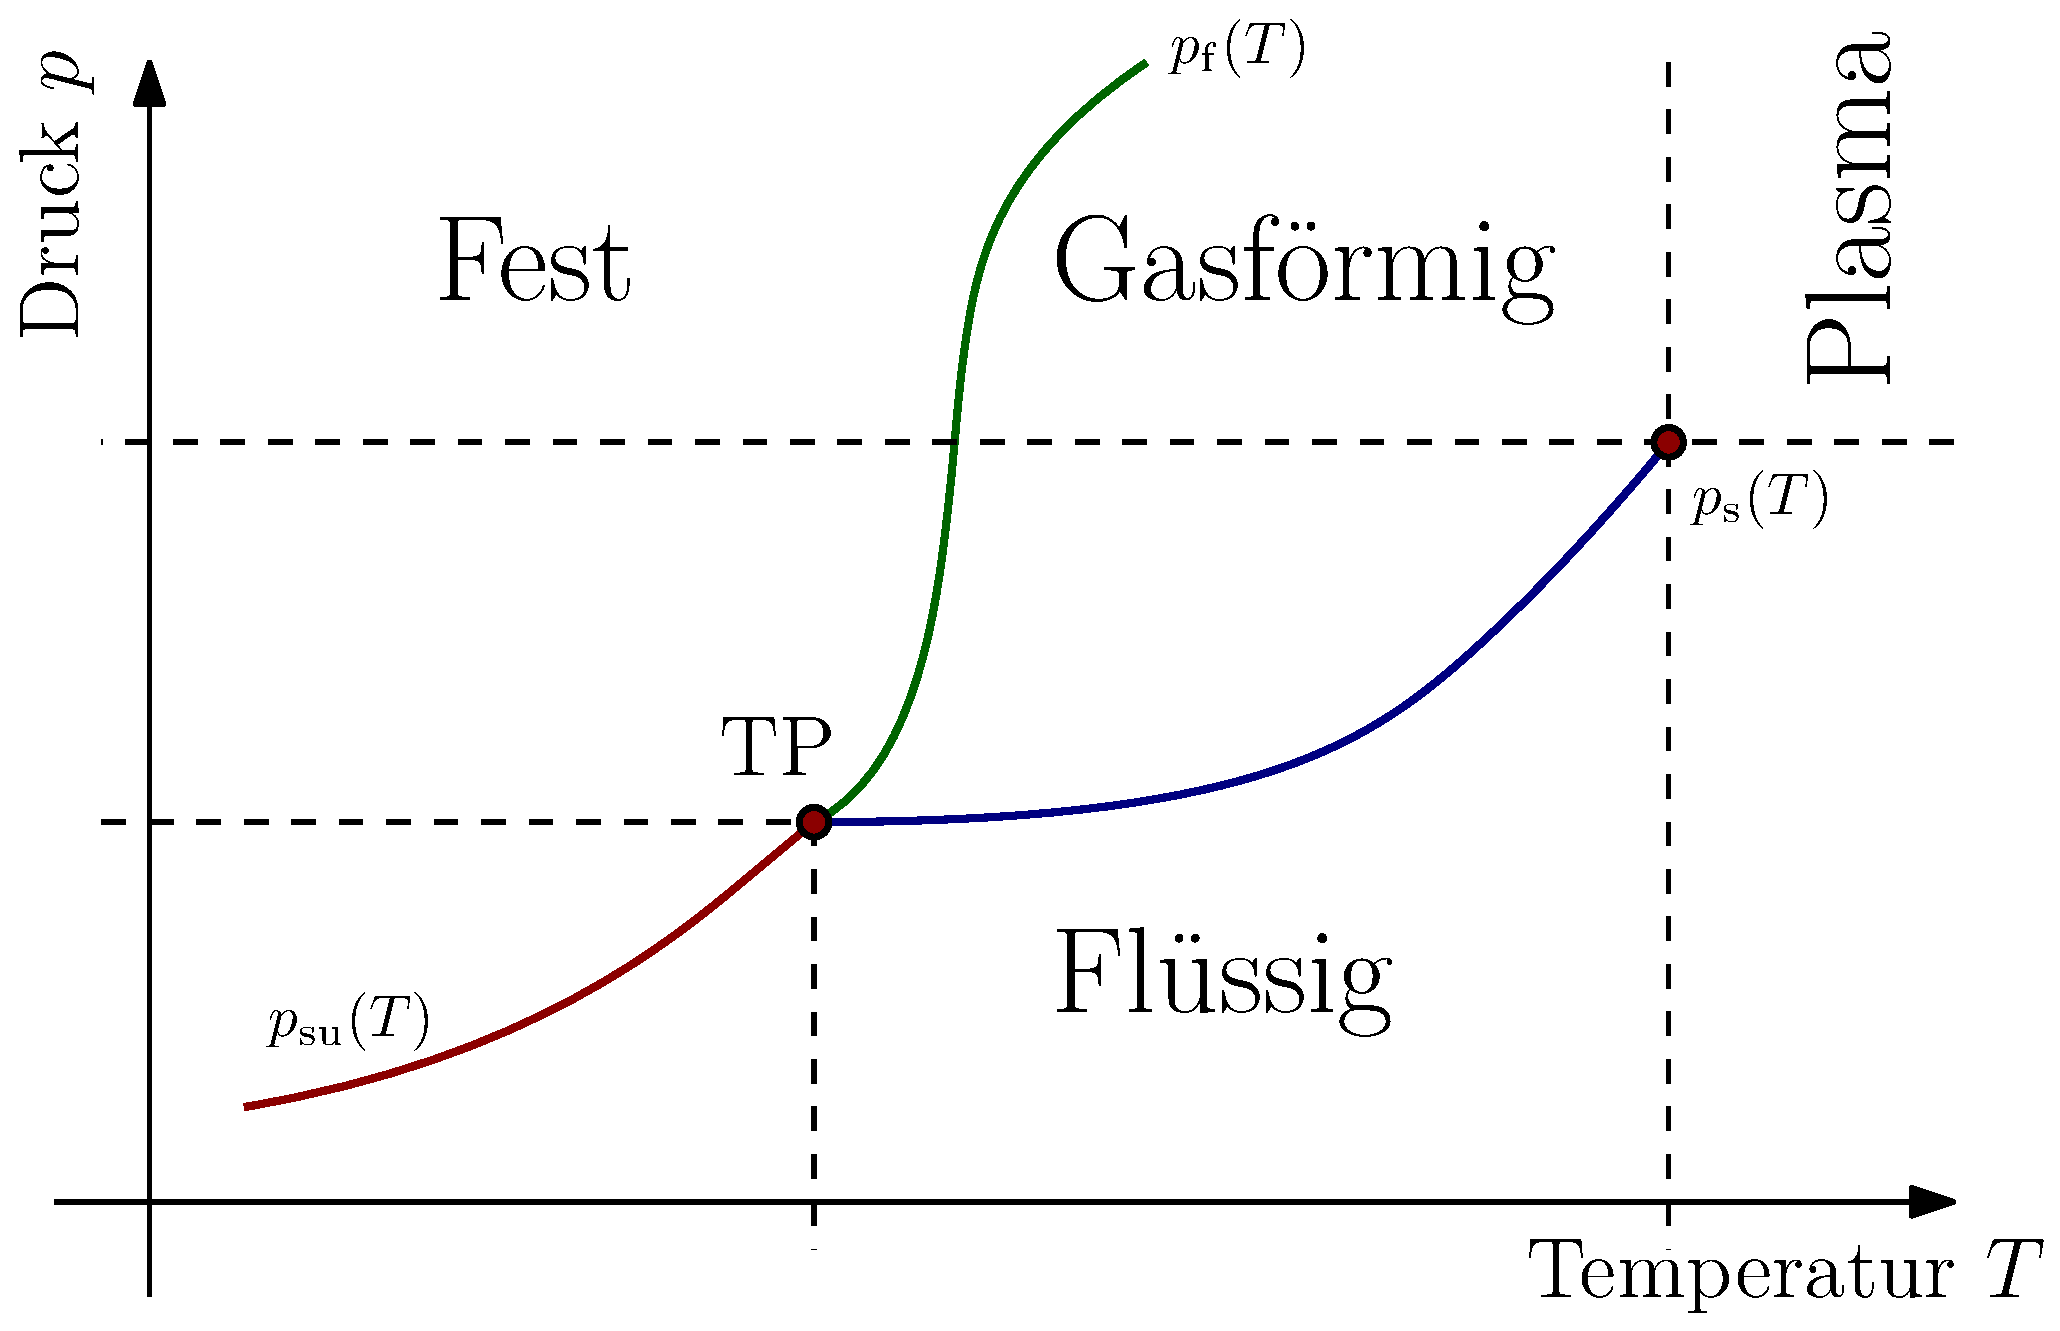
\includegraphics[width=\linewidth]{fig/phase-diagram}%
    \caption{\tt FIXME}
\end{figure}

\begin{definition}[Clasius-Clapeyron Gleichungen]
\[
    \deriv{p_\text{s}}{T} =
        \frac{q_\text{s}}{T\left(\varrho_g^{-1} - \varrho_f^{-1}\right)}
    \qquad
    \deriv{p_\text{f}}{T} =
        \frac{q_\text{f}}{T\left(\varrho_f^{-1} - \varrho_s^{-1}\right)}
\]
\begin{result}[Dampfdruck und Schmelzdruck]
\begin{gather*}
    p_s(T) = p_{s_0} \exp\left[
        \frac{q_s M_w}{R} \left(
            T_0^{-1} - T^{-1}
        \right)
    \right] \\
    p_f(T) = p_{s_0} \exp\left[
        \frac{q_f M_w}{R} \left(
            T_0^{-1} - T^{-1}
        \right)
    \right]
\end{gather*}
\end{result}

\begin{result}[Magnus Dampfdruck] Approximiert die L\"osung der Clasius-Clapeyron Differenzialgleichung f\"ur Wasser.
\[
    p_s(\vartheta) = p_{s_0}
        \exp_{10}\left({\frac{7.5\vartheta}{\vartheta + 265.5}}\right)
\]
\end{result}
\end{definition}

\begin{definition}[Taupunkt und Taupunktstemperatur]
Die Temperatur, bei der beim Abk\"uhlen feuchter Luft S\"attigungs erreicht wird und Kondensation einsetzt, wird \emph{Taupunkt} genannt.
\[
    p_D = p_s (\vartheta_d)
\]
\end{definition}

\begin{definition}[Luftfeuchtigkeit]
\(m_w\) ist die Masse des \emph{in der Luft enthaltenen} Wasserdampfes.
\(m_s\) ist die maximale Dampfmasse im S\"attigungszustand.
\(P_D\) ist die Partialdruck des Wassedampfes.
\begin{align*}
    \text{Absolute} \quad f   &= \frac{m_w}{V}                              & \unitof{f}   & = \unitof{\varrho} \\
    \text{Relative} \quad f_r &= \frac{m_w}{m_s} = \frac{p_D}{p_s} \leq 1 & \unitof{f_r} & = 1
\end{align*}
\end{definition}

\begin{definition}[Dichte des feuchten Luft]
\[
    \varrho_F = \varrho_T + \frac{p_D(M_w - M_L)}{RT}
        \quad \varrho_F < \varrho_T
\]
\end{definition}

\subsection{W\"armetransport \fromlecture{13}}

\begin{definition}[Fourier'sche Gesetz der W\"armeleitung]
\begin{gather*}
    j = \frac{\delta Q}{A\di{t}} \propto \deriv{T}{x}
    \implies
    j = -\lambda \deriv{T}{x}
    \\
    \unitof{j} = \si{\joule\per\square\metre\per\second} = \si{\watt\per\square\metre}
    \quad
    \unitof{\lambda} = \si{\watt\per\metre\per\kelvin}
\end{gather*}
\end{definition}


\subsection{Thermodynamische Prozesse \fromlecture{14}}

\subsection{Zustand\"anderungen}

\begin{definition}[Isobare]
\(
    p = \left(\text{konstant}\right)
\), folgt:
\begin{align*}
    \delta Q &= nC_{mp} \di{T} &
    \delta W &= p \di{V}
    \\
     Q &= nC_{mp} \Delta T &
     W &= p\Delta V = nR \Delta T
\end{align*}
\end{definition}

\begin{definition}[Isochore]
\(
    V = \left(\text{konstant}\right) \iff \dd{V} = 0
\), folgt:
\begin{align*}
    \delta Q &= nC_{mv} \di{T} &
    \delta W &= p \di{V} = 0
    \\
     Q &= nC_{mv} \Delta T &
     W &= 0
\end{align*}
\end{definition}

\begin{definition}[Isotherme]
\(
    T = \left(\text{konstant}\right) \iff \dd{T} = 0
\), folgt:
\begin{align*}
    \delta Q &= nC_{mv} \di{T} = 0 & 
    \delta W &= p \di{V}
    \\
     Q &= 0 &
     W &= nRT\ln\left(\frac{V_2}{V_1}\right)
\end{align*}
Weil:
\(\displaystyle
    W = \int \delta W 
    = \int\limits_{V_1}^{V_2} p \di{V}
    = \int\limits_{V_1}^{V_2} \frac{nRT}{V} \di{V}
\)
\end{definition}

\begin{definition}[Adiabatische Zustand\"anderungen] D.h. \emph{kein} W\"armeaustauch zwischen dem betrachteten System und seiner Umgebung stattfindet.

\end{definition}

\begin{thebibliography}{2}
\bibitem{hsr}
    \textsc{Hochschule f\"ur Technik Rapperswil (HSR)}.
    \textit{\texttt{Ph2HAT} Vorlesungen und die dazugeh\"orige Unterlagen,}
    Sourlier David,
    Fr\"uhlingssemester 2020,
    Rapperswil.

\bibitem{bucher-ruh}
    \textsc{Arthur Ruh, Benno Bucher}.
    \textit{Physik 1: Mechanik, Fluide, W\"armelehre}.
    Vol I, HSR, 2014, Rapperswil.

\bibitem{feynman1}
    \textsc{Richard Feynman}.
    \textit{Mainly Mechanics, radiation, and heat}.
    \textit{The Feynman Lectures on Physics},
    Leighton, Sands,
    New Millenium Edition,
    Vol I,
    Basic Books,
    California Institute of Technology (Caltech).

\bibitem{feynman2}
    \textsc{Richard Feynman}.
    \textit{Mainly electromagnetism and matter}.
    \textit{The Feynman Lectures on Physics},
    Leighton, Sands,
    New Millenium Edition,
    Vol II,
    Basic Books,
    California Institute of Technology (Caltech).

\end{thebibliography}


\section*{License}
{ \tt
Ph2HAT-ZF (c) by Naoki Pross
\\\\
Ph2HAT-ZF is licensed under a Creative Commons Attribution-ShareAlike 4.0 Unported License.
\\\\
You should have received a copy of the license along with this work. If not, see 
\\\\
{\small\url{http://creativecommons.org/licenses/by-sa/4.0/}}
}

\end{document}

% vim: set et sw=4 ts=4 wrap linebreak spell spelllang=de:
